\synctex=1

%%%%
%%%% Multiagent Simulation and the MASON Library
%%%% Copyright 2010 by Sean Luke
%%%%
%%%% LaTeX Source
%%%% This source code, and embedded PDFs and sources (such as OmniGraffle Files)
%%%% Are distributed under the Academic Free License version 3.0
%%%% See the file "LICENSE" for more information
%%%%
%%%% When you build this source code, the resulting PDF file is licensed under the
%%%% Creative Commons Attribution-No Derivative Works 3.0 United States License
%%%% See the URL http://creativecommons.org/licenses/by-nd/3.0/us/   for more information
%%%%
%%%% If you have any questions, feel free to contact me at sean@cs.gmu.edu
%%%% Sean Luke

\documentclass[twoside,10pt]{article}
\usepackage{fullpage}
\usepackage{mathpazo}
\usepackage[noend]{algpseudocode}
\usepackage{amsmath}
\usepackage{latexsym}
\usepackage{graphicx}
\usepackage{wrapfig}
\usepackage{bm}
\usepackage{qtree}
\usepackage{array}
\usepackage{eurosym}
\usepackage{textcomp}
\usepackage{makeidx}
\usepackage{rotating}
\usepackage{multirow}
\usepackage{multicol}
\usepackage{microtype}
\usepackage{afterpage}
\usepackage{color}\definecolor{gray}{gray}{0.5}
\usepackage{alltt}
\usepackage{tabto}
\usepackage[font=footnotesize,labelsep=quad,labelfont=it]{caption}
\usepackage{todonotes}

\usepackage{listings}		% distributed 
\usepackage{xcolor}			% distributed

%%% Added in order to use hyperref -- this stuff has to appear before bibentry,x
%%% which has a conflict with regard to \bibitem.  See later in this file for more stuff that has
%%% to be added afterwards
  \makeatletter
  \let\saved@bibitem\@bibitem
  \makeatother

\usepackage{bibentry}
\usepackage[hyperfootnotes=false,linktocpage=true,linkbordercolor={0.5 0 0}]{hyperref}
%%% Note that to avoid a link being created from \pageref, just use \pageref*
%%% End hyperref stuff

\renewcommand\textfraction{0.0}
\renewcommand\topfraction{1.0}
\renewcommand\bottomfraction{1.0}


\newcommand\file[1]{\textsf{#1}}
\newcommand\variable[1]{\textsf{#1}}
%\newcommand\package[1]{\textsf{#1}}
\newcommand\package[1]{\index{Packages!{#1}}\textsf{#1}}
\newcommand\Package[1]{\index{Packages!{#1}|textbf}\textsf{#1}}
%\newcommand\class[1]{\textsf{#1}}
\newcommand\class[1]{\index{Classes!{#1}}\textsf{#1}}
\newcommand\Class[1]{\index{Classes!{#1}|textbf}\textsf{#1}}
\newcommand\method[1]{\hbox{\textsf{#1}}}
\newcommand\parameter[1]{\texttt{#1}}
\newcommand\character[1]{\texttt{"{#1}"}}
\newcommand\textstr[1]{\texttt{"{#1}"}}
\newcommand\code[1]{\textsf{#1}}

\newcommand\ignore[1]{}


\newcommand\sidebara[3]{\begin{wrapfigure}{r}[0in]{3.2in}%
\vspace{-1.1em}\hfill\framebox{\begin{minipage}{3in}\setlength\parindent{1.5em}\footnotesize{\noindent\textit{#1}

\vspace{0.5em}{\noindent #2}}
\end{minipage}}
\vspace{#3}
\end{wrapfigure}
}

\newcommand\sidebar[2]{\begin{wrapfigure}{r}[0in]{3.2in}%
\vspace{-1.1em}\hfill\framebox{\begin{minipage}{3in}\setlength\parindent{1.5em}\footnotesize{\noindent\textit{#1}

\vspace{0.5em}{\noindent #2}}
\end{minipage}}
\vspace{-0.5em}
\end{wrapfigure}
}



%%% Hack to allow more spacing before and after an hline
\newcommand\tstrut{\rule{0pt}{2.4ex}}
\newcommand\bstrut{\rule[-1.0ex]{0pt}{0pt}}

% Increase the numbering depth
\setcounter{secnumdepth}{3}
\setcounter{tocdepth}{6}


%%%% This code is used to create consistent lists of methods

% From TUGboat, Volume 24 (2003), No. 2 "Hints & Tricks"
\newcommand*{\xfill}[1][0pt]{%
	\cleaders
		\hbox to 1pt{\hss
			\raisebox{#1}{\rule{1.2pt}{0.4pt}}%
			\hss}\hfill}
			
\newenvironment{methods}[1]{
\vspace{1.0em}\noindent\textsf{\textbf{#1 Methods}}\quad \xfill[0.5ex]
\vspace{-0.25em}
\begin{description}
\small}
{\end{description}\hrule\vspace{1.5em}}

\newcommand{\mthd}[1]{\item[{\sf #1}]~\newline}


\newcommand\booktitle{MASON Discrete Event Simulation Extension}
\newcommand\reference[1]{\vspace{0.5em}\hfill{\parbox{6in}{\raggedleft\noindent\textsf{#1}}}}

% Include subsubsection in the TOC
\setcounter{tocdepth}{3}

% Use with a %, like this:   \params{%
\newcommand\params[1]{\vbox{\begin{quote}\small\tt{\noindent{#1}}\end{quote}}}
\newcommand\script[1]{\params{#1}}
\newcommand\java[1]{\params{#1}}

% Allow poor horizontal spacing
\sloppy

% Allow a ragged bottom even in two-sided
\raggedbottom

% Command to push text to following page without the cutoff that occurs with clearpage
\newcommand\bump{\vspace{10in}}

% Command to push text to following line
\newcommand\hbump{\hspace{10in}}


% Define an existing word in text as an index item
\newcommand{\idx}[1]{\index{#1}#1}

% Define an existing word in text as an index item and make it bold
\newcommand{\df}[1]{\index{#1}\textbf{#1}}

% Provide a separate index item for a word in text and make it bold
\newcommand{\dfa}[2]{\index{#1}\textbf{#2}}

% Create algorithms and definitions
\newtheorem{algm}{Algorithm}
\newtheorem{defn}{Definition}

% Initial figures, pages, algorithms, and sections should be 0 :-)
\setcounter{figure}{-1}	% Mona is Figure 0
\setcounter{page}{-1}	% Start with Page 1 (the Front Page).  I'd like it to be Page 0 but it messes up twosided
\setcounter{algm}{-1}	% Start with Algorithm 0 (the Example Algorithm)
\setcounter{section}{-1}	% Start at Section 0 (the Introduction)

\thispagestyle{plain}
\thispagestyle{empty}

\newcommand\hsp[1]{{\rule{0pt}{0pt}\hspace{#1}}}
\newcommand\spc{{\rule{0pt}{0pt}~}}


%%%% Some stuff for Distributed

\lstdefinestyle{Bash}{
  language=bash,
  basicstyle=\small\sffamily,
  numbers=left,
  numberstyle=\tiny,
  numbersep=3pt,
  frame=tb,
  breaklines=true, 
  columns=fullflexible,
  backgroundcolor=\color{yellow!20},
  linewidth=0.9\linewidth,
  xleftmargin=0.1\linewidth
}

\definecolor{javared}{rgb}{0.6,0,0} % for strings
\definecolor{javagreen}{rgb}{0.25,0.5,0.35} % comments
\definecolor{javapurple}{rgb}{0.5,0,0.35} % keywords
\definecolor{javadocblue}{rgb}{0.25,0.35,0.75} % javadoc

\lstdefinestyle{CustomJava}{
    language=java,
    basicstyle=\ttfamily,
    keywordstyle=\color{javapurple}\bfseries,
    stringstyle=\color{javared},
    commentstyle=\color{javagreen},
    morecomment=[s][\color{javadocblue}]{/**}{*/},
    numbers=left,
    numberstyle=\tiny\color{black},
    stepnumber=2,
    numbersep=10pt,
    tabsize=2,
    showspaces=false,
    breaklines=true, 
    showstringspaces=false}





\makeindex


\begin{document}

\noindent\huge\bf \booktitle\\
\\
%{\large\rm A User Manual for the MASON Multiagent Simulation Toolkit}\\
\\
\Large\bf Sean Luke\\
{\large\rm 
Department of Computer Science\\
George Mason University}
\\
\\
\\
\large\rm {\bf Manual Version 2}\\
\large\rm June 2023\\

\clearpage



\normalsize
\cleardoublepage

\tableofcontents
\clearpage

\section{Introduction}

\subsection{Installing the DES Extension}

\subsection{What You Need to Know about MASON}

\subsection{About Discrete Event Simulation}

\subsection{About Hybrid ABM and DES Simulation}

\begin{figure}[t]
\centering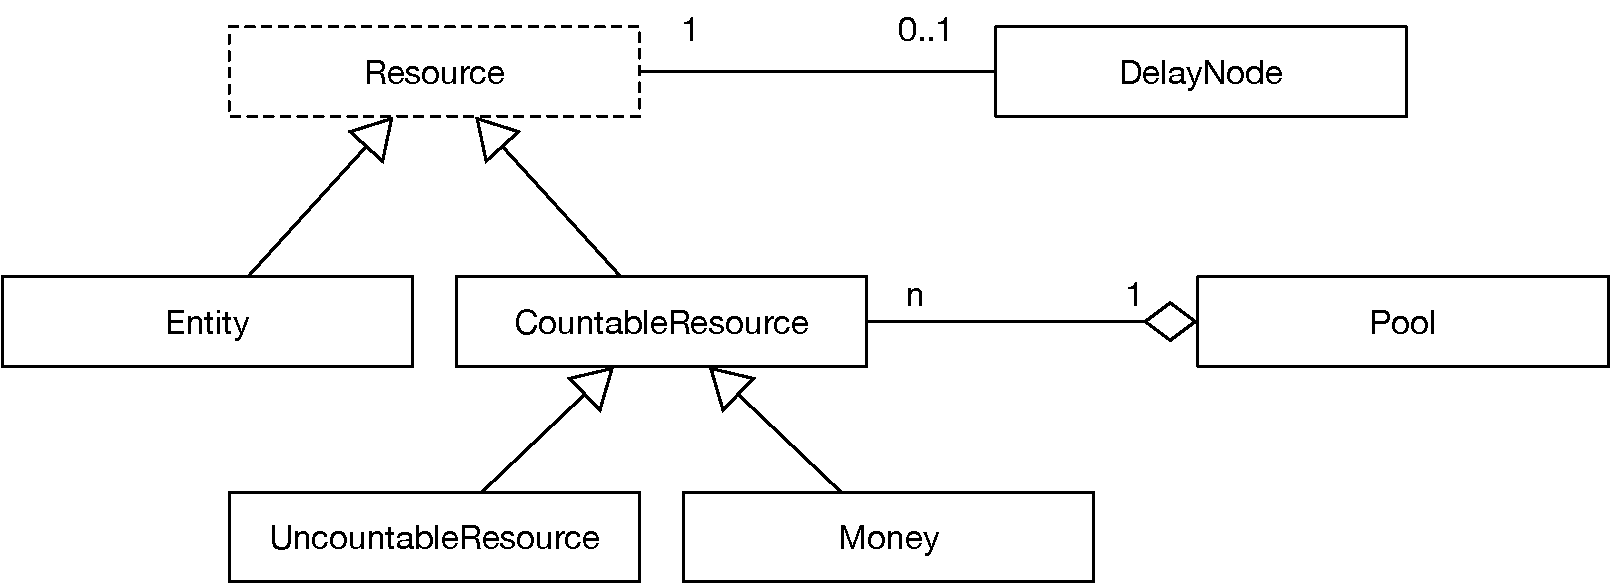
\includegraphics[width=4in]{Resources.pdf}
\end{figure}


\section{Resources}

The DES Extension has two basic kinds of classes:  {\bf Resources} and {\bf Processes}.   Processes perform actions in response to events.  In most cases, this action involves Processes handing off Resources to other Processes.  This could be for many reasons.  Perhaps a Resource moving from Process A to Process B to another represents A paying B for some service.  Perhaps Processes A and B are warehouses and the Resource represents a truck moving from one to the other.  Perhaps A and B are countries and the Resource represents a family migrating.  Maybe A and B are spies and the Resource holds a critical communication between them.

Resources are also held in {\bf Pools}.  A Pool can be dipped into by certain Processes to allocate a Resource for some temporary function.  For example, imagine if a factory floor had four assembly lines but only two lathes.  Widgets moving through an assembly line at some point had to be lathed, and if a lathe was not available, the widget (and its assembly line) would have to wait until one came available.

To do this, there are two special kinds of Processes, copies of which are part of each assembly line, called {\bf Lock} and {\bf Unlock}.  For a widget to pass through a Lock, the Lock must first allocate a Resource (representing the lathe) from a shared Pool.  If it cannot, the widget must wait until the Lock can allocate the Resource.  Then the widget may pass through to other Processes.  Ultimately when widget is finished with the lathe, the widget can pass through an {\bf Unlock} Process, which gives a Resource back to the Pool.   The Pool only holds two lathe Resources.\footnote{These are called Lock and Unlock because they are reminiscent of locking or unlocking on a mutex or a semaphore in computer science terminology.   So sue me, I'm a computer science professor. Others in the Discrete Event Simulation world might instead refer to {\bf seizing} and {\bf releasing} resources from a pool.}
  
MASON provides several kinds of Resources, depending on your modeling needs:

\begin{itemize}
\item {\bf Entities} are atomic elements, like tickets or tokens or cars.  They cannot be broken up into smaller Entities, nor joined together to form larger ones.  They are not worth different amounts: and Entity is an Entity.
\item {\bf Composite Entities} are Entities which hold a collection of other Resources inside them, plus a manifest.  For example, a Composite Entity might be used to model a shipping container filled with teddy bears.  The manifest can indicate anything you'd like: expiration dates, country of origin, who manufactured each bear, the amount of love that went into each bear, and so on.  There is a special Process called a {\bf Composer} which takes a collection of Resources and builds a Composite Entity 
\item {\bf Countable Resources} are Resources which can be divided, but only as integers.  For example, packages of medicine pills are countable resources: the package could be 0 pills, or 1 pill, or 2 pills, or 1500 pills.  But it cannot be 1.5 pills.  You cannot have a negative or infinite value.
\item {\bf Money} is an obvious example of a Countable Resource.  In US currency, the fundamental unit of money is the penny.  You cannot have a half a penny, and you cannot have 3.279 pennies.  Because money is so common, MASON has a dedicated kind of Countable Resource just to represent it: it prints it out in a pleasing fashion (like ``\$14.23'' for 1423 pennies). 
\item {\bf Uncountable Resources} are Resources which can be divided indefinitely.  An example of an uncountable resource is water.  You can have 3.239122 liters of water, and you can divide that into five parts any way you like, including some parts holding 0 liters.  You cannot have a negative or infinite value.
\end{itemize}

Resources are typed, and you can have as many different types of Resources as you like.  For example, you could have a type of Countable Resource representing pills and another one representing punches in the face.  You could have a type of Uncountable Resource representing water and another one representing love.  You could have both US dollars and Hong Kong dollars.  You could have both cargo containers and suitcases of stuff.  These types are not exchangeable: you can't give a Process water when it's expecting love.  However there exists a special Process, called a {\bf Transformer} which can convert certain Resources into Countable Resources: for example, it could be used as a currency converter.     

If Resources are typed, how do you make a new type of Resource, and how do you make more of that same type?  Each Resource type has a unique name.  To make a new type of resource, just instantiate a Resource class with that new name.  Later Resources of that type are allocated by copying them from earlier Resources of the same type. This can be done either by calling \method{duplicate()} or by calling a copy constructor on the earlier Resource, indicating the amount of the new Resource.

Processes deal with Resources differently based on the kind of Resources.  For example, many Processes store Resources to eventually hand off to downstream Processes.  If the Resource is an Entity, then it is atomic and the Process must store it in a collection of Entities.  If the Resource is a Countable or Uncountable Resource, then the Process can simply merge it into one pile or blob of Countable (or Uncountable) Resource, and dole it out as appropriate later on.

All Resources have {\bf amounts}.  For Countable or Uncountable resources, the amount is simply the size of the resource: such as 1500 pills or 1423 pennies or 3.239122 liters of water.  For Entities, including Composite Entities, the amount is always 1.

\subsection{Resource}

Resource is the abstract superclass of all resources.  All Resources have a {\bf unique type} (an integer) shared by resources of that type, and a {\bf name} (a String) which you can stipulate.  For example, all Electricity resources might have type 0, and all Gas resources might have type 1 and all Cars might have type 2 and all Dollars might have type 3.  It is possible to construct two Resources with the same name, but they will have different types even so: don't do that.  For your own sanity, make sure that you only construct a Resource once with a given name, and copy Resources from it to make more of the same type.

\begin{methods}{\class{sim.des.Resource} Constructor}
\mthd{public Resource(String name)}
Builds a new Resource, of a new unique type, with the given name.
\mthd{protected Resource()}
Builds a new Resource, but does not set the name or type.  This exists to permit copy constructors in subclasses.  Normally you'd leave it alone.
\end{methods}

\begin{methods}{\class{sim.des.Resource}}
\mthd{public void clear()}
Clears the resource. What this does varies depending on the subclass.
\mthd{public void toString()}
Prints the resource in a pleasing manner.
\mthd{public boolean equals(Object other)}
Returns true if {\it other} is a Resource, is not null, and if it is both the same type and amount as this Resource.  The storage and info elements inside Composite Entities are not checked for equality. 
\mthd{public int hashCode()}
Returns an appropriate hash code for hash tables.
\mthd{public double getAmount()}
Returns the amount of the Resource.  Note that this is always double, even for Countable Resources and for Entities, both of which return integers.
\mthd{public boolean isSameType(Resource other)}
Returns true if {\it other} is not null and the same type as this Resource. 
\mthd{public int getType()}
Returns the type of this resource. 
\mthd{public String getName()}
Returns the name of this resource. 
\mthd{protected void setName(String name)}
Sets the name of this resource.  You shouldn't call this probably.
\mthd{public Resource duplicate()}
Exactly duplicates the Resource once and returns the result.  The storage and info objects are not copied\,---\,just pointer-copies.  You'll have to deep copy them as you see fit.
\mthd{public Resource[] duplicate(int times)}
Exactly duplicates the Resource {\it times} times and returns the result.  The storage and info objects are not copied\,---\,just pointer-copies.  You'll have to deep copy them as you see fit.
\end{methods}


\subsection{Entity}

An Entity is a Resource that cannot be subdivided into smaller Resources of the same time.  For example: a Car might be an Entity.  But Water is not, as you can divide Water up into smaller amounts.  Entities can {\bf store} other resources inside them: that is, they can be {\bf composed} of them.  For example, a given Car might contain Wheels, and Engine, and some amount of Gasoline.  Different Cars are permitted to store different things.  Entities can also contain {\bf info} objects, essentially manifests.

\begin{methods}{\class{sim.des.Entity} Constructor}
\mthd{public Entity(String name)}
Builds a new Entity, of a new unique type, with the given name.
\mthd{public Entity(Entity other)}
Makes a copy of the Entity, including its type and name.  The storage and info objects are pointer-copied, not deep-copied.  This is the standard copy constructor for Entity.
\end{methods}

Here are the custom methods for Entity.  It also implements the methods defined in Resource.

\begin{methods}{\class{sim.des.Entity}}
\mthd{public Resource[] getStorage()}
Returns the actual storage array of the Entity, or null if there isn't one.
\mthd{public void setStorage(Resource[] val)}
Sets the storage array of the Entity.  This can be set to null.
\mthd{public Object getInfo()}
Returns the actual info object of the Entity, or null if there isn't one.
\mthd{public void setInfo(Object val)}
Sets the info object of the Entity.  This can be set to null.
\mthd{public boolean isComposite()}
Returns true if the storage is non-null.
\mthd{public void clear()}
Sets the storage to null.
\mthd{public double getAmount()}
Always returns 1.0.
\mthd{public boolean equals(Object other)}
Returns true if {\it other} is an Entity, is not null, and if it is the same type as this Entity.  The storage and info elements inside Composite Entities are not checked for equality. 
\mthd{public int hashCode()}
Returns an appropriate hash code for hash tables, not considering the storage or info elements.
\end{methods}

\subsection{CountableResource}

A CountableResource is a Resource that has an {\bf amount} (an integer) and can be subdivided into CountableResources with smaller integer amounts.  For example: a Population might be divided into smaller subpopulations.  There is an atomic, smallest, non-divisible amount of CountableResources: 1.  You can also set the amount to 0.

Even though CountableResource only stores integers for amounts, it stores them as doubles.  This means that its maximum integer value is larger than that of an int.  Specifically, it is equal to \variable{sim.des.CountableResource.MAXIMUM\_INTEGER}

\begin{methods}{\class{sim.des.CountableResource} Constructor}
\mthd{public CountableResource(String name, double intialAmount)}
Builds a new CountableResource, of a new unique type, with the given name and amount.
\mthd{public CountableResource(String name)}
Builds a new CountableResource, of a new unique type, with the given name and zero amount.
\mthd{public CountableResource(CountableResource other)}
Makes a copy of the CountableResource, including its type, name, and amount.  If the provided object is actually an UncountableResource, this will throw an exception.
\mthd{public CountableResource(CountableResource other, double intialAmount)}
Makes a copy of the CountableResource, including its type and name, but with the new amount provided.    If the provided object is actually an UncountableResource, this will throw an exception.
\end{methods}

Here are the custom methods for CountableResource.  It also implements the methods defined in Resource.

\begin{methods}{\class{sim.des.CountableResource}}
\mthd{public double doubleValue()}
Returns the amount as a double value.
\mthd{public boolean isUncountable()}
Returns false (note that this is overridden by UncountableResource).
\mthd{public boolean isCountable()}
Returns true (note that this is overridden by UncountableResource).
\mthd{public double getAmount()}
Returns the amount stored in the CountableResource, which will always be a nonnegative integer (but possibly larger than an int).
\mthd{public void clear()}
Sets the amount to 0.
\mthd{public double getAmount()}
Returns the amount.
\mthd{public void setAmount(double val)}
Sets the amount
\mthd{public void bound(double min, double max)}
Bounds the resource to be no more than max and no less than min.  It must be the case that max \(\geq\) min \(\geq\) 0.
\mthd{public void bound(double max)}
Bounds the resource to be no more than max and no less than zero.  It must be the case that max \(\geq\) 0.
\mthd{public boolean increase(double val)}
Increases the amount by the given value and returns true, unless val is not an integer, or unless this would exceed \variable{sim.des.CountableResource.MAXIMUM\_INTEGER}, in which case nothing happens and false is returned.
\mthd{public boolean decrease(double val)}
Decrements the amount by the given value and returns true, unless val is not an integer, or unless this would drop below zero, in which case nothing happens and false is returned.
\mthd{public boolean increment()}
Increments the amount by 1 and returns true, unless this would exceed \variable{sim.des.CountableResource.MAXIMUM\_INTEGER}, in which case nothing happens and false is returned.
\mthd{public boolean decrement()}
Decrements the amount by 1 and returns true, unless this would drop below zero, in which case nothing happens and false is returned.
\mthd{public CountableResource reduce(double atLeast, double atMost)}
Subtracts at least a certain amount and at most a certain amount from this CountableResource, placing that amount into a new CountableResource and returning it, unless there is not enough amount to do so, in which case nothing happens and false is returned.  atLeast and atMost must be integers, with atMost \(\geq\) atLeast \(\geq\) 0.
\mthd{public CountableResource reduce(double byExactly)}
Subtracts exactly a certain amount from this CountableResource, placing that amount into a new CountableResource and returning it, unless there is not enough amount to do so, in which case nothing happens and false is returned.  byExactly must be an integer \(\geq\) 0.
\mthd{public void add(CountableResource other)}
Adds the other CountableResource's amount into this one, setting the other CountableResource's amount to zero afterwards.
\mthd{public void add(CountableResource other, double atMostThisMuch)}
Adds atMostThisMuch of the other CountableResource's amount into this one, setting the other CountableResource's amount to the remainder afterwards.
\mthd{public void add(CountableResource[] other)}
Adds all the other CountableResources' amounts into this one, setting the other CountableResources' amounts to zero afterwards.
\mthd{public boolean greaterThan(CountableResource other)}
Returns true if this amount is greater than the other resource's amount.
\mthd{public boolean greaterThanOrEquals(CountableResource other)}
Returns true if this amount is greater than or equal to the other resource's amount.
\mthd{public boolean lessThan(CountableResource other)}
Returns true if this amount is less than the other resource's amount.
\mthd{public boolean lessThanOrEquals(CountableResource other)}
Returns true if this amount is less than or equal to the other resource's amount.
\mthd{public int compareTo(Object other)}
Returns 0 if the other object's amount is equal to, -1 if it is greater than, and 1 if it is less than my amount. 
\end{methods}



\subsection{Money}

Money is a CountableResource with a cute printing function which prints it with a currency sign.  For example, a Dollar is Money, hence a CountableResource, where the smallest amount (1) would be the Cent.  Perhaps it should be renamed Cents.

\begin{methods}{\class{sim.des.Money} Constructor}
\mthd{public Money(String name, double intialAmount)}
Builds a new Money, of a new unique type, with the given name and amount.  The name will be used as a currency symbol during printing.
\mthd{public Money(String name)}
Builds a new Money, of a new unique type, with the given name and zero amount.   The name will be used as a currency symbol during printing.
\mthd{public Money(Money other)}
Makes a copy of the Money, including its type, name, and amount.
\mthd{public Money(Money other, double intialAmount)}
Makes a copy of the Money, including its type and name, but with the new amount provided.
\end{methods}

Here are the custom methods for Money.  It also implements the methods defined in CountableResource.

\begin{methods}{\class{sim.des.Money}}
\mthd{public String toString()}
Returns the amount in decimal format as \(CX.Y\), where \(C\) is the name (a currency symbol), \(X\) is the amount / 100, and \(Y\) is the amount mod 100.  For example, if ``\$'' was the name, and the amount was 1423, then this would print as ``\$14.23''
\end{methods}


\subsection{UncountableResource}

An UncountableResource is a CountableResource which can be subdivided infinitely and has real-valued amounts.  Thus while you can only have a CountableResource with values 0, 1, 2, 3, ...., an UncountableResource could be any positive amount, such as 0 or 2.34129 or 92.3 or Infinity.

If you have a variable holding a CountableResource, how do you know it is a CountableResource versus an UncountableResource?  You could use {\tt instanceof}, or you could call {\tt isCountable()} or {\tt isUncountable()}.

\begin{methods}{\class{sim.des.UncountableResource} Constructor}
\mthd{public UncountableResource(String name, double intialAmount)}
Builds a new UncountableResource, of a new unique type, with the given name and amount.
\mthd{public UncountableResource(String name)}
Builds a new UncountableResource, of a new unique type, with the given name and zero amount.
\mthd{public UncountableResource(UncountableResource other)}
Makes a copy of the UncountableResource, including its type, name, and amount.
\mthd{public UncountableResource(UncountableResource other, double intialAmount)}
Makes a copy of the UncountableResource, including its type and name, but with the new amount provided.
\end{methods}

Here are the custom methods for UncountableResource.  It also implements the myriad of methods defined in CountableResource.

\begin{methods}{\class{sim.des.UncountableResource}}
\mthd{public UncountableResource[] divide(int times)}
Divides the amount by {\it times}, which must be \(> 0\), and builds {\it times} \(-1\) new UncountableResources, each with the new amount.  Also reduces the amount of this UncountableResource to the amount as well. 
\mthd{public UncountableResource halve()}
Builds a new UncountableResources with half the amount, leaving the other half as the current amount.
\mthd{public void scale(double value)}
Changes the amount by multiplying it by the given value.
\mthd{public boolean increase(double val)}
Increases the amount by the given value and returns true.
\mthd{public boolean decrease(double val)}
Decrements the amount by the given value and returns true, unless this would drop below zero, in which case nothing happens and false is returned.
\end{methods}




\subsection{Pool}

A {\bf Pool} is a storage of a single kind of CountableResource, UncountableResource, or Money.   Various Process objects, namely {\bf Lock} and {\bf Unlock}, dip into a shared Pool to add or remove resources or to wait until resources have come available.

Pool is very simple: it has a {\bf maximum} amount of resource, a {\bf minimum} (always zero), and an {\bf initial resource allocation}.   Beyond that, its current resource can be set and queried.  And that's it!

A Pool extends \class{sim.des.portrayal.DESPortrayal}, so it can serve as a MASON SimplePortrayal.  DESPortrayal objects are also \class{sim.des.Named}, so the Pool can be given a name via \method{getName()} and \method{setName(...)}.

A Pool is \class{sim.des.Resettable}, meaning that it can be reset to its original state via a method called \method{reset(...)}.


\begin{methods}{\class{sim.des.Pool} Constructor}
\mthd{public Pool(CountableResource resource, double maximum)}
Builds a Pool of the given type of CountableResource, with an initial amount copied from the CountableResource, and the provided maximum.
\mthd{public Pool(CountableResource resource)}
Builds a Pool of the given type of CountableResource, with an initial amount copied from the CountableResource, and a maximum of infinity (if it's an UncountableResource), or \variable{CountableResource.MAXIMUM\_INTEGER} (if it's a CountableResource or Money).
\mthd{public Pool(double initialResourceAllocation)}
Builds a Pool of a new type of CountableResource, with an initial amount as specified, and a maximum of infinity (if it's an UncountableResource), or \variable{CountableResource.MAXIMUM\_INTEGER} (if it's a CountableResource or Money).
\mthd{public Pool(double initialResourceAllocation, double maximum)}
Builds a Pool of a new type of CountableResource, with an initial amount as specified, and the specified maximum.
\end{methods}

A Pool only has a few methods:

\begin{methods}{\class{sim.des.Pool}}
\mthd{public void reset(SimState state)}
Resets the Pool.   This simply resets its current amount to the initial amount: the name and maximum stay as you had last set them.
\mthd{public CountableResource getResource()}
Returns the current available resource.
\mthd{public void setResource(CountableResource val)}
Sets the current available resource.
\mthd{public double getMaximum()}
Returns the maximum allowed resource.
\mthd{public void setMaximum(double value)}
Sets the maximum allowed resource.
\mthd{public String getName()}
Returns the name (which can be null).
\mthd{public void getName(String name)}
Sets the name (which can be null).
\mthd{public String toString()}
Returns the Pool and its state in a pleasing fashion.
\end{methods}


\clearpage
\begin{figure}[t]
\centering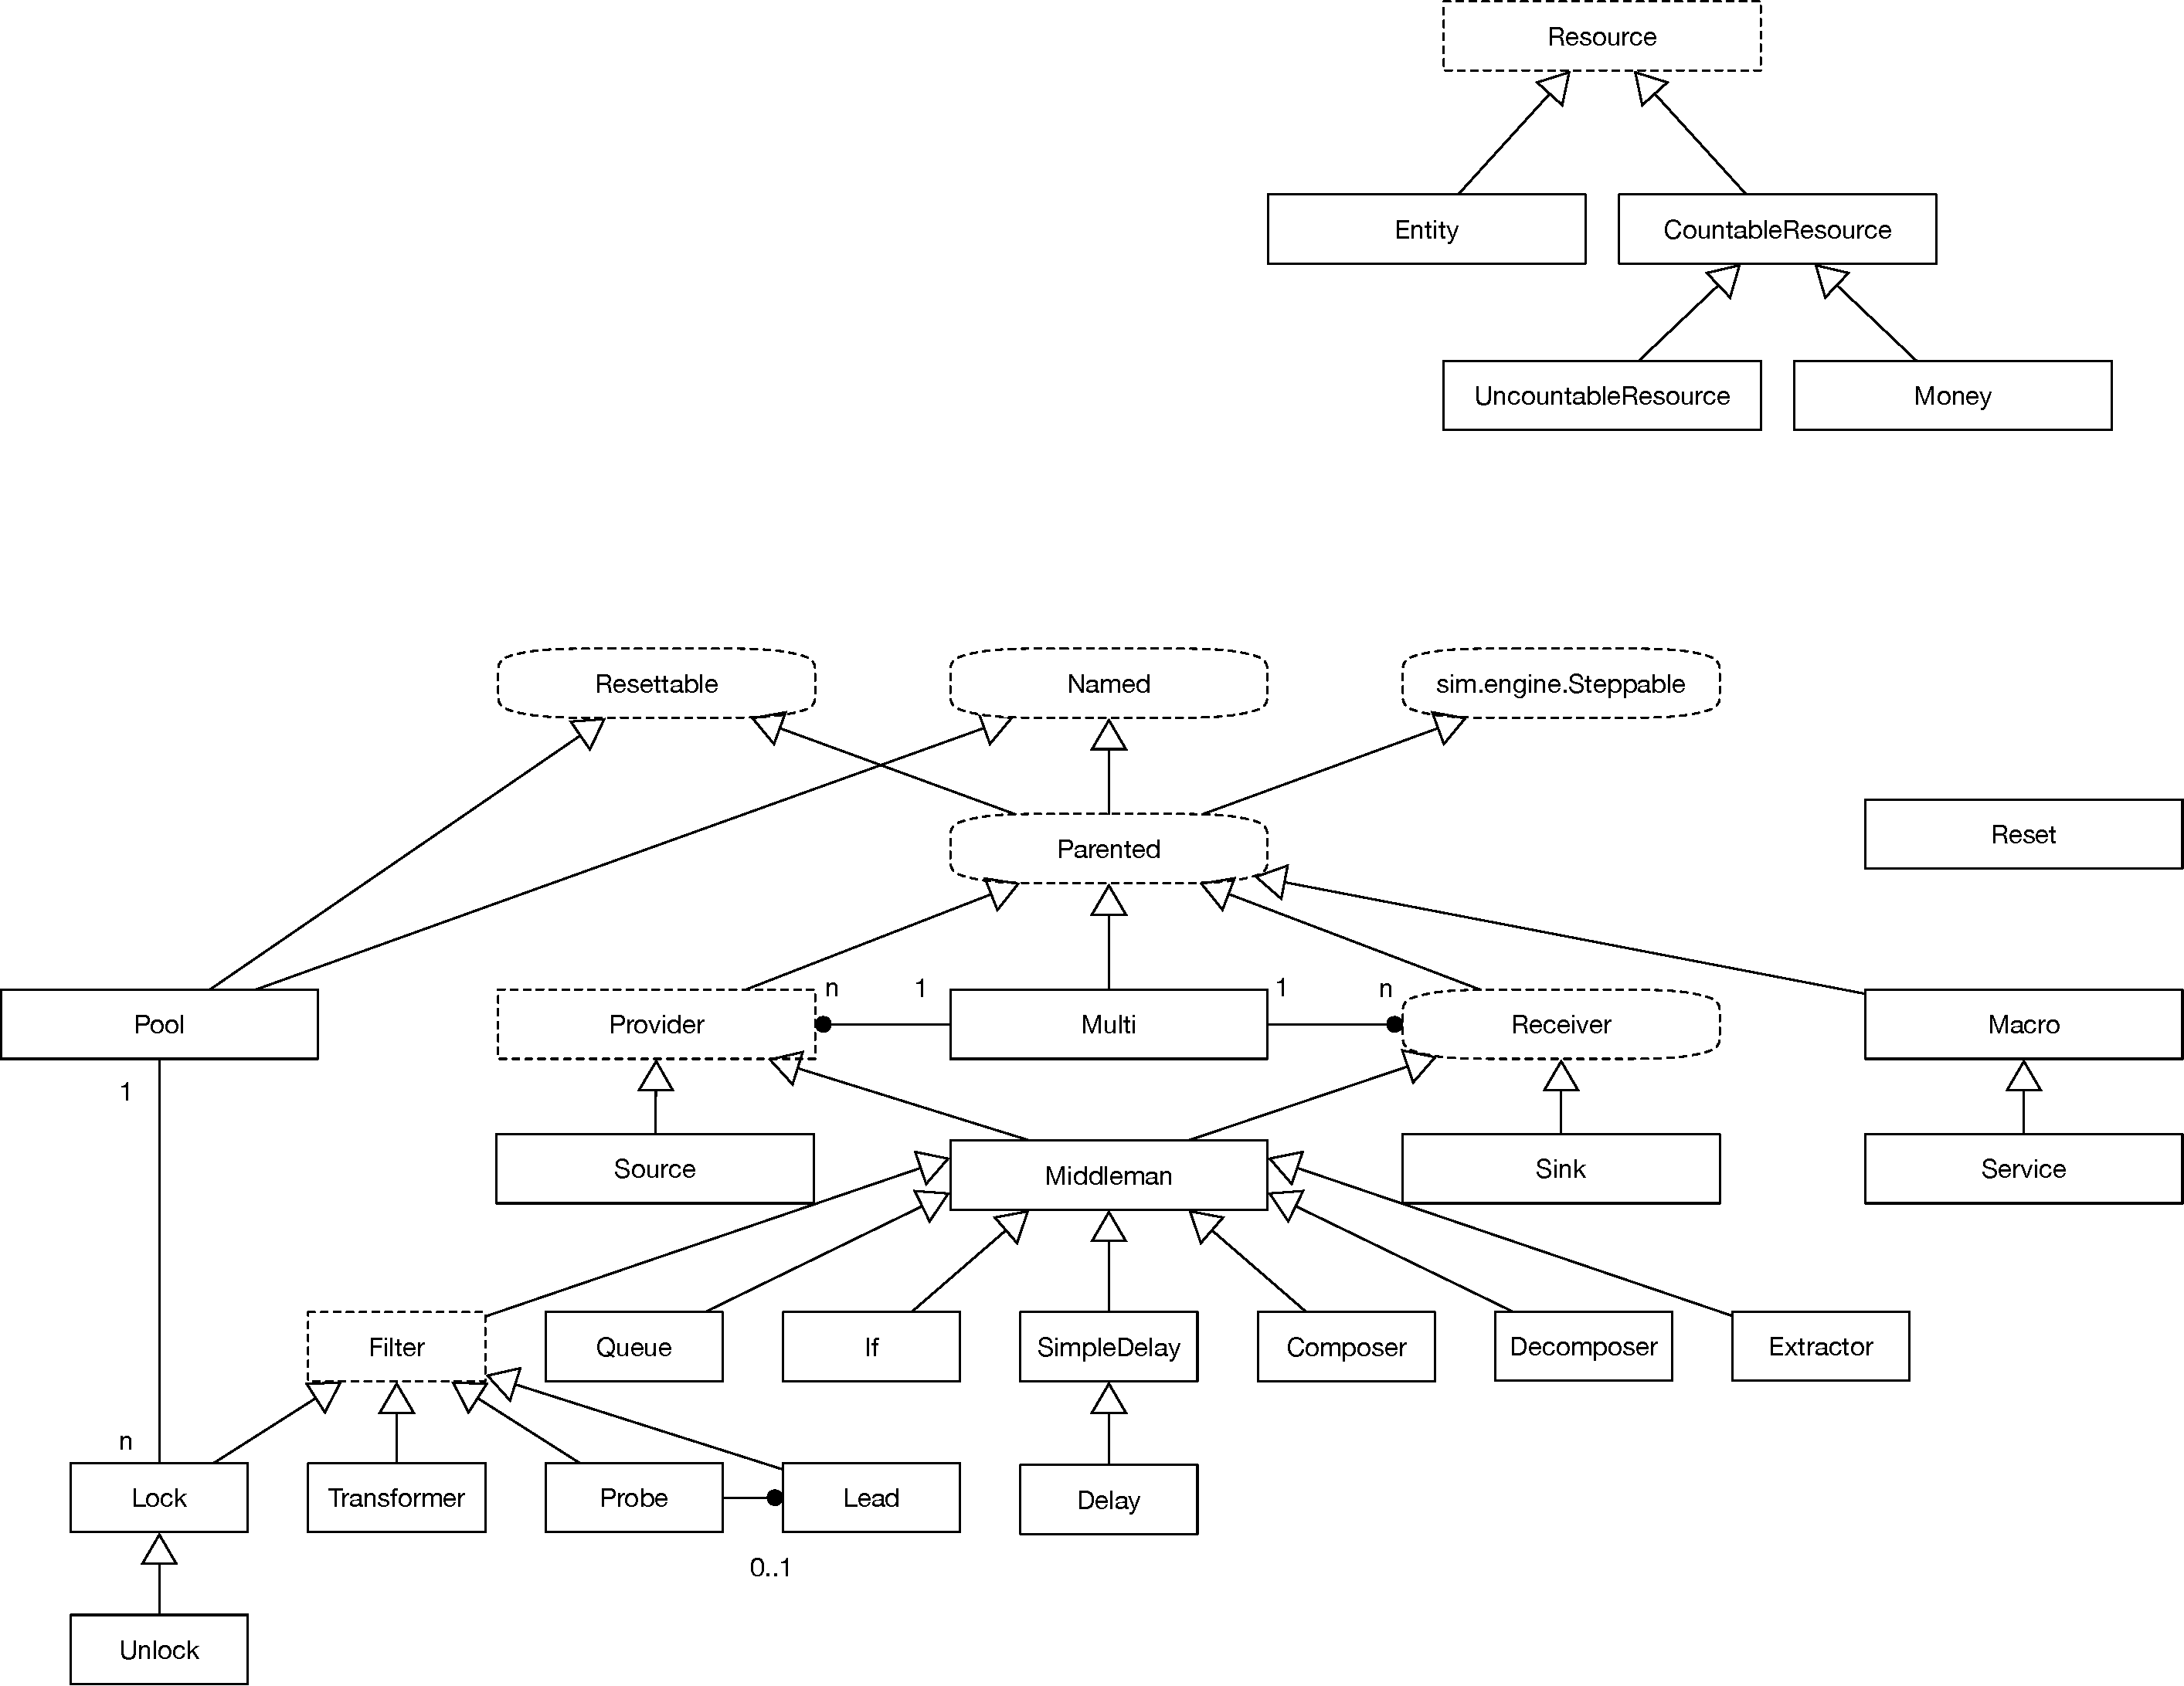
\includegraphics[width=6.5in]{Processes.pdf}
\end{figure}

\section{Processes}

Processes are the verbs of the DES system.  They perform actions in response to {\it events} (or if you like, {\it signals}) they receive.  

An event can be one of two things typically:

\begin{itemize}
\item Another Process can {\it offer} some Resources to the Process.
\item Another Process can {\it request} that the Process offer it a resource.
\item Another Process can {\it offer a transaction} (an exchange) of a Resource for some other Resource.
\item MASON's Schedule can send an event to the Process to wake it up to do some work.
\end{itemize}



Various Process objects can be {\bf Receivers} or {\bf Providers} or both, or compose these objects into groups using the {\bf Macro} and {\bf Multi} classes.  Some Process objects can be placed on MASON's schedule to be stepped when appropriate. Other Processes do not require the schedule to pass work through them and onto other Processes.

The Processes, and support objects, implement a few interfaces.

\subsection{sim.engine.Steppable}

An object which can be placed on MASON's schedule to be stepped in the future.  All processes are Steppable, but only a few need it. [Perhaps in the future we should be more selective in this regard].

\subsection{Named}

An object which has a {\bf name} (a String).

\subsection{Parented}

An object which can be part of a parent process.  For example, Macros may contain many Parented objects within them, and are their parents.

\subsection{Resettable}

An object which can be {\bf reset} by a {\bf Reset} object.

\subsection{Reset}

Collects a bunch of {\bf Resettable} objects and allows you to easily {\bf reset} all of them.  This way you can create your DES graph in the model's constructor, then reset it each time you {\bf start()} the model, by just calling {\bf reset()} on your Reset in the body of the start() method.

\subsection{Provider}

An object which can make offers to one or more Receivers.  Receivers are {\bf registered} with the Provider.  When the Provider has a resource to offer, it will go to each of its Receivers according to some {\bf offer policy} and ask them to {\bf accept} offers of the Resource until it is depleted.  Providers can also be asked by a Receiver to make an offer to it.    Providers have a {\bf typical Resource type} of the resource that they offer.  Rarely, a Provider can provide more than one resource.

\subsection{Receiver}

An object which can {\it receive} an offer from a Provider.  That is, the Provider will offer the Receiver some amount of Resource, asking it to {\bf accept} the offer.  Offers have minimum and maximum amounts that the Receiver may select from.  The receiver accepts some appropriate amount (between the min and max) of the Resource being offered by the Provider, or it refuses it.  A Receiver can also go to a Provider and {\bf ask} that the Provider make an offer to the Receiver.  Receivers have a {\bf typical Resource type} of the resource that they accept.  Rarely, a Receiver can receive more than one resource.

\subsection{Sink}

A Receiver which accepts all offers (of the appropriate Resource type) and throws the resulting Resource away.  {\bf By default, this class's step() method does nothing, so there's no need to schedule it.}

\subsection{Source}

A Provider which generates Resources and offers it to downstream registered Receivers.  You can customize your Source however you want, but the default form works as follows.  Each time the Source is ready to {\bf produce} some Resource, the amount it produces is determined either by a {\bf distribution} or a {\bf deterministic amount}.  It then adds this Resource to a pile, and offers all the Resources currently in the pile to its receivers.  Sources have a maximum {\bf capacity} for their pile and will not generate more than this.  After making offers, the Source then uses {\it another} distribution or deterministic amount to determine the {\bf next time} it will generate Resources and make offers.  It schedules itself appropriately.


\subsection{MiddleMan}

An object which is both a Provider and a Receiver.  You can make your own Provider+Receiver combination, but MiddleMan is a nice abstract superclass.  

\subsection{Extractor}

Both a Receiver and a Source (sort of).  An Extractor is works like a Source, except that it ``builds'' its resources by extracting them from another Provider.  You could, for example, attach an Extractor to a Queue and every once i a while the Extractor would pull out of the Queue and offer resources to downstream Receivers.  Extractors ignore capacity.

\subsection{Queue}

Both a Receiver and Provider.  When a Queue receives a Resource, it adds it to a pile, then (usually) immediately offers this pile to its own receivers.  The Queue's pile has a maximum capacity.  If it cannot add to the pile, it will refuse the offer.

\subsection{SimpleDelay}

Both a Receiver and Provider.  When a SimpleDelay receives a Resource, it adds it to a linked list and, after a delay of some fixed amount of time, then offers the Resource to downstream receivers.  If the receivers do not accept, then the Resource is discarded.  The SimpleDelay has a maximum capacity of items it may store which are presently delayed.

\subsection{Delay}

A subclass of SimpleDelay.  This is just like a SimpleDelay, except that the delay time for each object received can be {\it different}, so some Resources can move through the Delay faster than others.  Thus the SimpleDelay is implemented using a heap rather than a linked list.

\subsection{Composer}

Both a Receiver and Provider.  Upon receiving a Resource, it adds it to a collection of Resources. These Resources can be of different types.  When it has all the necessary amounts of Resources for each type, it gathers them together and produces a Composed Entity holding these Resources, then offers the Entity to downstream receivers. If they do not accept, then the Entity is discarded.  The Composer has both minimum and maximum (capacity) amounts for each of the Resources needed to compose into the Entity.

\subsection{Decomposer}

Both a Receiver and Provider.  Upon receiving a Composed Entity, it decomposes it and offers each of its Resources to various downstream receivers, one registered for each Resource type. If they do not accept, then that Resource is discarded.  {\bf By default, this class's step() method does nothing, so there's no need to schedule it.}

\subsection{If}

A Middleman which receives and incoming offer, then chooses only one of several possible Receivers to hand the offer to.  This choice is specified in a method defined by the modeler.


\section{Filters}

Filters are just Processes which accept offers and immediately turn around and offer them to a single downstream Receiver.  Filters are both Providers and Receivers, and never respond to requests to make offers.

\subsection{Filter}

The abstract superclass of Filters, which simply gathers together variables and methods common to them.

\subsection{Transformer}

Upon receiving a Resource, Transformer {\bf transforms} the Resource into a different one according to a certain rule, then immediately offers it to downstream receivers.  If they do not accept, then the Resource is discarded.  {\bf By default, this class's step() method does nothing, so there's no need to schedule it.}

\subsection{Lock}

Upon receiving a Resource, Lock attempts to {\bf allocate} some amount of {\it a different} Resource from a {\bf Pool}.  If successful, it then offers the original Resource to downstream receivers. If they do not accept, then that Resource is discarded.  {\bf By default, this class's step() method does nothing, so there's no need to schedule it.}

\subsection{Unlock}

A subclass of Lock, but only for convenience's sake.  Upon receiving a Resource, it {\bf provides} some amount of {\it a different} Resource to a {\bf Pool}.  Regardless of whether the Pool accepts this generosity, Unlock then offers the original Resource to downstream receivers. If they do not accept, then that Resource is discarded.  {\bf By default, this class's step() method does nothing, so there's no need to schedule it.}

\subsection{Probe}

An object which gathers statistics on the resources which pass through it.  A Probe can also be used in conjunction with a {\bf Lead}.

\subsection{Lead}

An object detached from Probe with can be used in combination with it to determine the amount of resources in a DES subgraph between them.

\section{Process Utilities}

\subsection{Macro}

An object which can store a {\bf subgraph} of the DES graph.  This subgraph consists of some {\bf Receivers}, some {\bf Providers}, and some {\bf in-between Processes}.  When stepped, the Macro steps all of its stored objects in order.  You can access the Receivers and Providers to make offers or register stuff as you see fit.

\subsection{Service}

A simple example of a common Macro consisting of a Lock, then a SimpleDelay, then an Unlock.




%\cleardoublepage
%\footnotesize
%\addcontentsline{toc}{chapter}{Index}
%\printindex

\end{document}














